%load balancing
\subsection{Dynamic Load Balancing Overview}

The overall aim of parallelising the FLAME framework is to reduce the wall clock time for running a simulation. This relies on efficient parallelisation of communication and keeping the work load balanced between computing nodes. The message board library addresses the first of these and dynamic load balancing addresses the second.

To illustrate the problems in getting load balancing right the diagram in Figure \ref{fig:load_balance_problem} shows agents on two nodes and their communication patterns. The top portion shows an unbalanced number of agents but the frequent communication is internal to each node with only infrequent communication between the nodes. If agents are moved to try to balance the load then frequent communication between nodes is introduced (lower portion of figure) which could mean a large increase in communication time and hence wall clock time. 

This example shows that measurement of communication between nodes must be part of the load balancing algorithm as well as elapsed time for various parts of the framework.

\begin{figure}[h]
 \centering
  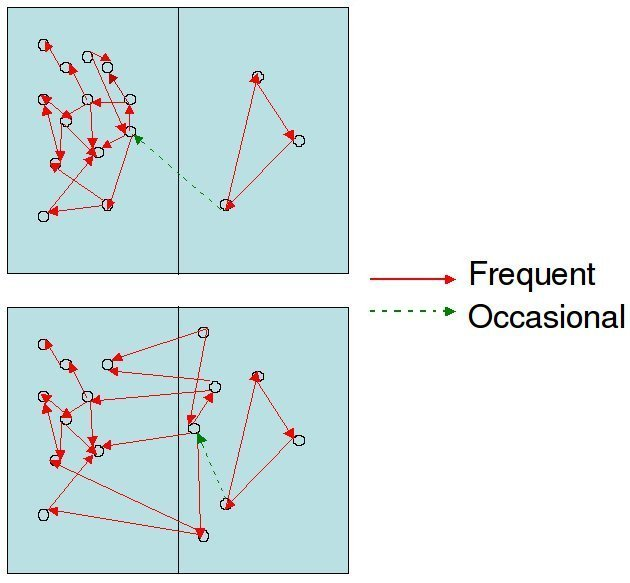
\includegraphics[scale=0.50]{load_balance.jpg}
 \caption{Illustrating some problems of load balancing}
 \label{fig:load_balance_problem}
\end{figure}

This section describes our initial thoughts on dynamic load balancing. The implementation has started with a timer which allows developers to insert timing into any section of FLAME from the framework itself to the user's model functions. It will be timing of different parts of the framework (which includes calls to the user's functions) that provides data for algorithms that seek to balance computational load.

\subsection{The \textit{timer} Package}

Timers will be used to measure the elapsed CPU time for portions of the running code and this data will be used as input to the load balancing strategy used in the FLAME framework. The initial requirements against which the timer package was implemented are given below.

\begin{itemize}
\item Can have multiple timers running simultaneously
\item Timers can be identified individually
\item Functions to start/stop/reset a named timer
\item Function to get elapsed time from a named timer
\item Definition of a set of timers.
\item Functions to get statistics from a set of timer
\item Turn timing on/off during program execution 
\end{itemize}

We have implemented all the functionality for individual timers and a set of unit tests and an example program using the timers. Code is stored under Subversion source code control in the FLAME project on the CCPForge site. 

User documentation is supplied in \cite{TimerAPI}.
